\documentclass{article}
\usepackage{graphicx}

\title{Classes}
\author{Miguel Flores-Acton}
\date{Fall 2024}

\begin{document}

\maketitle

\section{Schedule}
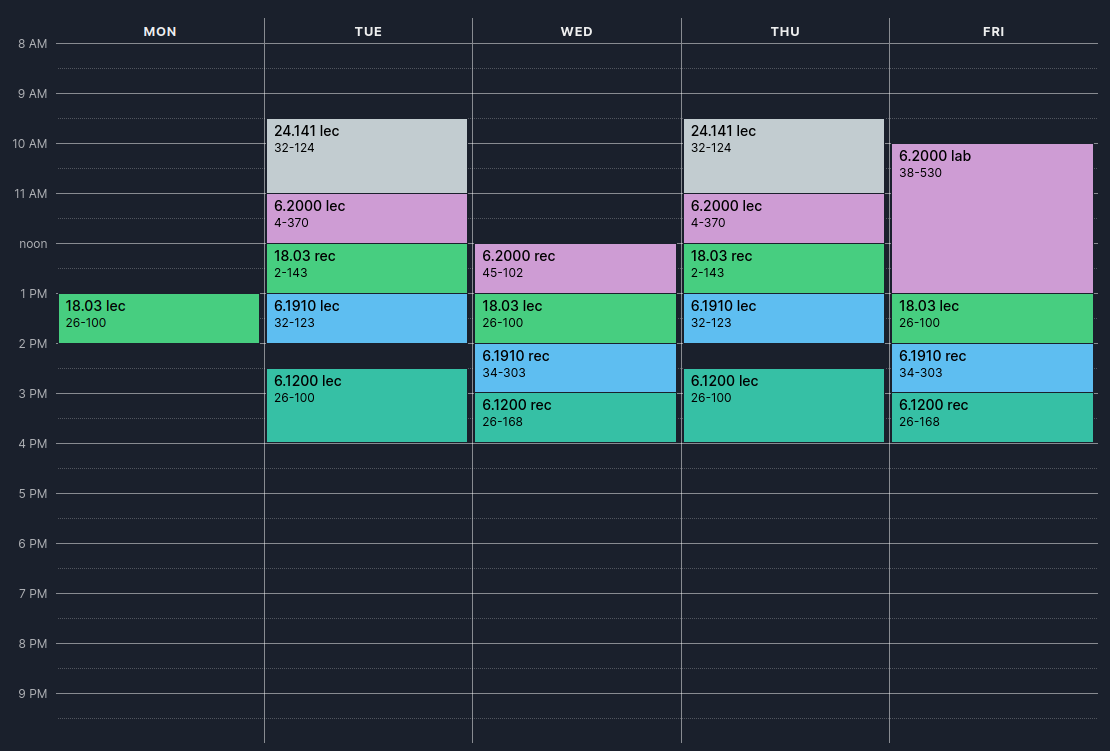
\includegraphics[width=1\textwidth]{image.png}

\section{Differential Equations - 18.03}
\textbf{Canvas \& MITx \& Gradescope}
\newline
9 PSets - 40\% total - 5\% each (lowest dropped)

Part A on MITx and Part B written on gradscope
\newline
3 Midterms - 30\% total - 10\% each
\newline
Final - 30\% total
\newline
Cutoff - A:90\% - B:80\% - C:70\% - D:60\%
\section{Logic 1 - 24.141}
\textbf{Canvas \& Carnap}
\newline
12 PSets - 50\% total - 5\% each (lowest two dropped)

- Due each Friday
\newline
Midterm - 20\% total
\newline
Final - 30\%
\newline
Cutoff - A:90\% - B:80\% - C:70\% - D:60\%
\section{Intro Circuits - 6.2000}
\textbf{CAT-SOOP}
PSets - 15\%
\newline
Labs - 15\%
\newline
Nano Quizez - 5\%
\newline
Midterm - 25\%
\newline
Final - 40\%
\newline
(Optional) Recitation Participation - 5\% taken out of exams
\newline
Cutoff - A:90\% - B:80\% - C:70\% - D:60\%

Must have D or higher in PSets, Labs, \& exams (weighted average of midterm and final)

\section{Computation Structures - 6.1910}
\textbf{Canvas}
Labs - 7 total - 80pts
\newline
Lecture Questions and Recitation attendance - 10pts
\newline
Quizzes - 3 total - 90pts
\newline
(Optional) Design Project - 20pts
\newline
Cutoff - A:165pts - B:145pts - C:125pts

Must complete all labs


\section{Discrete Math for Computer Science - 6.1200}
\textbf{Canvas \& Gradescope}


\section{Practical Signal Processing - ES.S31}
TBD

\end{document}
